\documentclass[aer.tex]{subfiles}
\begin{document}

\section{Transmitter}
The transmitter detects spike events and transmits
them out of the core (e.g. to a router or a receiver) in serialized AER
packets. Neurons are arranged in a 2D grid of rows (y address) and columns 
(x address). 
When a neuron spikes, it (and any other neuron in the same row) raises a 
request to the arbiter at the end of the rows. 
The row arbiter selects a row of neurons to transmit. The 
y address is then transmitted. Any neuron that spiked in the 
selected row then send their column addresses to the column latch and arbiter.
Their column addresses are latched to allow the neurons to reset while the 
column arbiter sequences the transmission of their x addresses. Once all of the
x addresses have been transmitted, the tail bit is transmitted to signal the 
end of the packet.

\subsection{Transmitter Decomposition}
Here we will start from a high level description of the transmitter and then decompose
the description into a set of concurrent, parallel processes. 
The highest level description of the address-event transmitter $AEXT$ is

\begin{csp}
AEXT(n)\equiv*[[\langle\|\,j:1..n:#{P`j}->A!enc(j)\pll\,P`j\rangle]]
\end{csp}
where 

\begin{tabular}[]{rl}
$n$ & is the number of neurons \\
$P_j$ & is the port communicating with the $j$th neuron \\
$A$ & is the output port \\
$enc(\cdot)$ & is a function returning the address of a neuron \\
\end{tabular} \\

In words, when the $j$th neuron spikes, output its address and reset the neuron. 
We rely on the "$\vert$" arbitration operator to handle multiple neurons spiking simultaneously.
We first expand $AEXT$ into rows and columns.

\begin{csp}
AEXT(x,y)\equiv*[[\langle\|\,l:1..y:\langle|k:1..x:#{P`{l\cdot\,k}}\rangle->A`1!enc(l)
               ,[\langle\|\,k:1..x:#{P`{l\cdot\,k}}->A`2!enc(k),P`{l\cdot\,k}\rangle]\rangle]]
\end{csp}
where 

\begin{tabular}[]{rl}
$x$ & is the number of columns \\
$y$ & is the number of rows \\
$P_{l\cdot k}$ & is the port communicating with the $l\cdot\,k$ neuron, and $\l\cdot k=xl+k$  \\
$A_1$ & is the row address output port \\
$A_2$ & is the column address output port \\
\end{tabular} \\

In words, for every row, wait for any neuron in that row to spike.
When a neuron spikes within a row, transmit the row address. In parallel,
arbitrate between the spiked neurons in the row 
and transmit one neuron's column addresses while resetting it.

We still rely on the arbitration operator, 
so our next step is to decompose $AEXT$ into separate processes for 
arbitration ($ARB$) and concurrent transmition ($ARY$). The arbitration process is given by

\begin{csp}
ARB(m)\equiv*[[\langle\|j:1..m:#{L`j}->L`j;L`j\rangle]]
\end{csp}
where $m$ is the number of processes to arbitrate and $L_j$ is port communicating with the $j$th process.
The first $L_j$ communication informs the $j$th process it may proceed, 
and the second $L_j$ communication confirms when the $j$th process has finished 
before the arbiter moves on to the next process. 
With the arbiter defined, we define the concurrent transmition process

\begin{csp}
ARY(y,x)\equiv*[[\langle,l:1..y:\langle|k:1..x:#{P`{l\cdot\,k}}\rangle->R`l;A`1!enc(l)
             ,[\langle,k:1..x:#{P`{l\cdot\,k}}->C`k;A`2!enc(k),P`{l\cdot\,k};C`k\rangle];R`l\rangle]]
\end{csp}
where

\begin{tabular}[]{rl}
$R_l$ & is the port communicating with the row arbiter \\
$C_k$ & is the port communicating with the column arbiter \\
\end{tabular} \\

From $AEXT$ to $ARY$, we replace arbitration "$\vert$" with concurrancy "$,$" and
introduce communications with the row and column arbiters.
As $ARB$ has two communications with each client: one to grant permission and one to check for 
completion, $ARY$ has two communications with the each arbiter: one to request permission and
one to indicate completion.

Next, we split out the address encoding function of $ARY$ into its own process.

\begin{csp}
ENC(m)\equiv*[[\langle[]j:1..m:#{L`j}->A!enc(j),L`j\rangle]]
\end{csp}

where $L$ communicates with $ARY$. We can use selection, which assumes mutual exclusion, 
in the encoding process because the arbiters ensure that we only attempt to encode one address at time.
Introducing a row and column address encoder, we rewrite $ARY$ as

\begin{csp}
ARY(y,x)\equiv*[[\langle,l:1..y:\langle|k:1..x:#{P`{l\cdot\,k}}\rangle->R`l;A`l
             ,[\langle,k:1..x:#{P`{l\cdot\,k}}->C`k;D`k,P`{l\cdot\,k};C`k\rangle];R`l\rangle]]
\end{csp}

where the $A_l$ port communicates with the row address encoder
and the $D_k$ port communicates with the column address encoder.

Next, we decompose $ARY$ into concurrent row and column processes.

\begin{csp}
ROW(x)\equiv*[[\langle|k:1..x:#{P`k}\rangle->R;
            A,[\langle,k:1..x:#{P`k}->C`k,P`k\rangle];R]]
COL(y)\equiv*[[\langle[]l:1..y:#{R`l}->C;D,R`l;C\rangle]]
\end{csp}

where

\begin{tabular}[c]{rl}
$P_k$ & communicates with the $k$th neuron in a row \\
$R$ & communicates the the row arbiter \\
$A$ & communicates with the row address encoder \\
$C_k$ & communicates with the $k$th column process \\
$R_l$ & communicates with the $l$th row process \\
$C$ & communicates with the column arbiter \\
$D$ & communicates with the column address encoder \\
\end{tabular}

In words, we have decomposed $ARY$ into $y$ $ROW$ processes and $x$ $COL$ processes. 
When a neuron spikes, its $ROW$ process makes a request to the row arbiter.
Once granted permission, $ROW$, in parallel, communicates with the row address encoder, 
signals the $COL$ processes corresponding to spiked neurons in the row to proceed, 
and sends reset signals to the spiked neurons.
When the row addess encoder, $COL$ processes, and neuron resets have completed, 
$ROW$ signals the row arbiter that it has finished.
The $COL$ processes use selection between the $R_l$ ports in the column because the 
row arbiter has ensured that only one $ROW$ process will signal the $COL$ process
at a time. 

Once signaled by a $ROW$ process, $COL$ makes a request to the column arbiter.
After gaining permission, $COL$ communicates with the column address encoder while
acknowledging the $ROW$ process. Finally, $COL$ signals the column arbiter that 
it has finished.

Our final step is to read out the activated columns in a row in parallel
and transmit the row and column addresses sequentially.
To read out columns in parallel, we modify $ROW$ and convert $COL$ into $LTH$ and $BUS$.
To sequence the address transmitions, we create $SEQ$.

$ROW$ is modified as

\begin{csp}
ROW(x)\equiv*[[\langle,k:1..x:#{P`k}->w.k+\rangle];R;
           A,C!w,[\langle,k:1..x:w.k->P`k\rangle];R,w:=0]
\end{csp}

where

\begin{tabular}[c]{rl}
$w$ & is an $x$-bit integer indicating which neurons spiked \\
$C$ & interfaces with $BUS$ (see below) \\
\end{tabular}

Note how $w$ is cleared at the end of the process as well. 
$BUS$ and $LTH$ are defined as

\begin{csp}
BUS(y,x)\equiv*[[\langle[]l:1..y:#{R`l}->C!(R`l?)\rangle]]
LTH(x)\equiv*[R?w;[\langle,k:1..x:w.k->C`k;D`k,w.k-;C`k\rangle];R]
\end{csp}

where for $BUS$,

\begin{tabular}[c]{rl}
$R_l$ & interfaces with an instance of $ROW$ \\
$C$ & interfaces with $SEQ$ (see below) \\
\end{tabular}

and for $LTH$

\begin{tabular}[c]{rl}
$R$ & interfaces with $SEQ$ \\
$C_k$ & interfaces with an the column $ARB$ \\
$D_k$ & interfaces with an instance of $ENC$ \\
\end{tabular}

$BUS$ simply communicates data between $ROW$ and $SEQ$. 
$LTH$ reads in data from $SEQ$ and sends the column addresses to be encoded.
The second $R$ communication indicates that all column addresses have been encoded.

$SEQ$ sequences the events

\begin{csp}
SEQ(b,x)\equiv*[S!(D?),T!(R?);S;T!\phi\]\pll*[T!(C?)]
\end{csp}

where 

\begin{tabular}[c]{rl}
$D$ & reads in data from $BUS$ \\
$S$ & communicates with $LTH$ \\
$R$ & interfaces with the row $ENC$ \\
$C$ & interfaces with the column $ENC$ \\
$T$ & is the transmitter output port \\
$\phi$ & is a reserved keyword for a tailword \\
\end{tabular}

The second $S$ communication corresponds to $LTH$'s second $R$ communication and
indiciates that the latch is empty and that the transmitter may move on to the next row.
There is a timing assumption that row data arrives at $T$ before column data.
This assumption is valid because the row data has fewer processes to traverse
than column data before reaching $T$.

Now that we have decomposed the transmitter, we will proceed to HSE and PRS
for the decomposed components.

%%%%%%%%%%%%%%%%%%%%%%%%%%%%%%%%%%%%%%%%%%%%%%%%%%%%%%%%%%%%%%%%%%%%%%%%%%%%%%%
\subsection{Event Generator (EVT)}
EVT interfaces the neuron with the rest of the transmitter. 
There is one EVT per neuron.
EVT has the following ports:

\begin{tabular}[]{rll}
  \code{P} & (passive) & communicates with the neuron \\
  \code{R} & (active) & communicates with row interface INT \\
  \code{C} & (active) & communicates with the column latch LTH \\
\end{tabular} \\ \\

EVT's HSE is given by

\begin{hse}
*[[pi];ro+;[ri];co+,po+;
 [~pi];ro-;[~ri];co-,po-]
\end{hse}  

In words,

\begin{tabular}[]{rl}
  \code{[pi]} & wait for the neuron to spike \\
  \code{ro$\uparrow$;[ri]} & get permission from the arbiter interface / row arbiter to go ahead \\
  \code{co$\uparrow$,po$\uparrow$} & send the column signal and the neuron reset signal \\
  \code{[$\neg$pi]} & wait for the neuron to reset \\
  \code{ro$\downarrow$;[$\neg$ri]} & indicate that the row arbiter can select the next row. \\
  \code{co$\downarrow$, po$\downarrow$} & reset the column request and neuron reset signals \\
\end{tabular} \\ \\

Note that the \code{[$\neg$ri]} wait also indicates that the sequencer is done with this row 
(and acknowledges \code{co$\uparrow$}). EVT's PRS is given by 

\begin{prs2}
 pi&~ri->ro+
~pi->ro-

 ri&ro->co+,po+
~ri->co-,po-
\end{prs2}
The \code{ro$\uparrow$} guard is strengthened with 
\code{$\neg$ri} so that if the neuron spikes immediately after it has
reset, \code{[$\neg$pi]}, 
we do not try to raise \code{ro} while executing \code{ro$\downarrow$}. 
The \code{co$\uparrow$,po$\uparrow$} guard is strengthened with \code{ro} because \code{ri} is a wire connecting all EVT instances in a row. We only want the neurons that have actually spiked
to proceed with raising their column and neuron reset lines.

\emph{The \code{co$\uparrow$} transition is not explicitely acknowledged. 
I hope this is accounted for by \code{$\neg$ri}...Check this after implementing LTH.}

Next, we explicitly represent the isochronic fork between
\code{co} and \code{ro} using a local variable \code{u}.
To make the PRS CMOS-implementable, we invert the sense of \code{pi}, \code{co}, and \code{po}.

\begin{prs2}
 ~_pi & ~ri -> ro+
_pi         -> ro-

u  -> _co-
~u -> _co+

 ri & ro -> u-
~ri      -> u+

u  -> _po-
~u -> _po+
\end{prs2}

Initially, \code{$\neg$po$\land\neg$ro$\land\neg$co} is true. With reset circuitry,

\begin{prs2}
~sReset & ~_pi & ~ri -> ro+
pReset | _pi -> ro-

u  -> _co-
~u -> _co+

_sReset & ri & ro -> u-
~_pReset | ~ri -> u+

u  -> _po-
~u -> _po+
\end{prs2}

%%%%%%%%%%%%%%%%%%%%%%%%%%%%%%%%%%%%%%%%%%%%%%%%%%%%%%%%%%%%%%%%%%%%%%%%%%%%%%%
\subsection{Interface (INT)}

There are two sets of INTs in the transmitter:
one for the rows and another for the columns.
The row INTs communicate with 
EVT, the row arbiter, and the y-address controller (ADY).
The column INTs communicate with 
the column address latch (LTH), the column arbiter, and the x-address controller (ADX).
Each row (column) INT has the following ports:

\begin{tabular}[]{rll}
  \code{V} & (passive) & receives requests from EVT (LTH) \\
  \code{C} & (active) & transmits request to the row (column) arbiter \\
  \code{E} & (active) & communicates with the row (column) address controller \\
\end{tabular} \\ \\

For row INTs, \code{vi} is the wired-or output of all EVT \code{ro} ports in the row. Likewise,
\code{vo} is connected to all of the EVT \code{ri} ports in the row.

INT's HSE is given by

\begin{hse}
*[[vi];co+;[ci&~ei];eo+,vo+;
 [~vi&ei];co-;[~ci];eo-,vo-]
\end{hse}

In words,

\begin{tabular}[]{rl}
  \code{[vi]} & wait for a request from EVT (LTH) for the arbiter \\
  \code{co$\uparrow$} & send request to arbiter \\
  \code{[ci$\land\neg$ei]} & wait for arbiter to grant permission and address controller to finish previous transmission \\
  \code{eo$\uparrow$, vo$\uparrow$} & \specialcell[t]{l}{
  signal EVT to transmit column information (LTH to transmit column addresses) \\
  signal address latch to store address } \\
  \code{[$\neg$vi$\land$ei]} & \specialcell[t]{l}{
    wait for EVT to reset neuron (LTH to send column address) \\
    and ADY (ADX) to have latched the address} \\
  \code{co$\downarrow$;[$\neg$ci]} & release arbiter \\
  \code{eo$\downarrow$, vo$\downarrow$} & return EVT and ADY (LTH and ADX) signals to initial value \\
\end{tabular} \\ \\

Note how INT signals the address encoder first after gaining permission from the arbiter
and second after the arbiter has been released instead of before the arbiter has been released.
This is safe because INT waits until \code{ei} clears before the first \code{E} communication. 
That is, \code{E} follows a lazy-active protocol.
INT's PRS is given by

\begin{prs2}
 vi      -> co+
~vi & ei -> co-

 ci & ~ei -> eo+, vo+
~ci       -> eo-, vo-
\end{prs2}

Next, we represent the isochronic fork between \code{eo} and \code{vo}
using local variable \code{y}. 
To make the PRS CMOS-implementable, we introduce local variable \code{x} and
invert the sense of \code{vi} and \code{ei}.

\begin{prs2}
vi         -> x-
~vi & ~_ei -> x+

ci & _ei -> y-
~ci      -> y+

y  -> eo-
~y -> eo+

~x -> co+
x  -> co-

y  -> vo-
~y -> vo+
\end{prs2}

Initially, \code{$\neg$co$\land\neg$vo$\land\neg$eo} is true. With reset circuitry,

\begin{prs2}
_sReset & vi          -> x-
~_pReset | ~vi & ~_ei -> x+

_sReset & ci & _ei -> y-
~_pReset | ~ci     -> y+

y -> eo-
~y -> eo+

~x -> co+
x -> co-

y -> vo-
~y -> vo+
\end{prs2}

%%%%%%%%%%%%%%%%%%%%%%%%%%%%%%%%%%%%%%%%%%%%%%%%%%%%%%%%%%%%%%%%%%%%%%%%%%%%%%%
\subsection{Arbiter (ARB)}

The arbiter cell ARB sequences requests from rows or columns by arbitrating between concurrent requests. 
Each ARB instance handles requests from two children and sends requests to its parent. 
To arbitrate between $N$ children, we use $N-1$ ARB cells arranged in a binary tree.
ARB is designed to be greedy but fair.
ARB's CHP is derived from

\begin{csp}
ARB\equiv*[[#{L`1}->R;L`1;L`1;R
          \|#{L`2}->R;L`2;L`2;R]]
\end{csp}

where

\begin{tabular}[c]{rl}
$L_1$ & communicates with the first child \\
$L_2$ & communicates with the second child \\
$R$ & communicates with the parent arbiter \\
\end{tabular}

The arbitration operator can be broken out into its own process

\begin{csp}
ARB\equiv\! *[[#{L`1}->A`1;R;L`1;L`1;R;A`1]]
      \pll*[[#{L`2}->A`2;R;L`2;L`2;R;A`2]]
      \pll*[[#{A`1}->A`1;A`1\|#{A`2}->A`2;A2]]
\end{csp}

The 2-way arbiter has ports:

\begin{tabular}[]{rll}
  \code{R} & (active) & transmits request to parent \\
  \code{L1} & (passive) & receives requests from left child 1 \\
  \code{A1} & (local) & request 1 to internal arbitration circuit \\
  \code{R1} & (local) & or'ed with \code{R2} to produce \code{R} \\
  \code{L2} & (passive) & receives requests from left child 2 \\
  \code{A2} & (local) & request 2 to internal arbitration circuit \\
  \code{R2} & (local) & or'ed with \code{R2} to produce \code{R} \\
\end{tabular} \\ \\

The existing HSE for the arbiter cell is given by

\begin{hse}
*[[l1i&~ri];a1o+;r1o+;[ri&a1i];l1o+;
  [~l1i];a1o-;r1o-;[~a1i];l1o-]

*[[l2i&~ri];a2o+;r2o+;[ri&a2i];l2o+;
  [~l2i];a2o-;r2o-;[~a2i];l2o-]
\end{hse}

In words, for the process communicating with the first child,

\begin{tabular}[]{rl}
  \code{[l1i$\land$~ri]} & wait for a child's request and to not already have the parent's go-ahead \\
  \code{a1o$\uparrow$} & request permission from the arbiter circuit \\
  \code{r1o$\uparrow$} & request permission from the parent \\
  \code{[ri$\land$a1i]} & wait for permission from the parent and arbiter circuit \\
  \code{l1o$\uparrow$} & signal child to go-ahead \\
  \code{[$\neg$l1i]} & wait for child to finish \\
  \code{a1o$\downarrow$} & withdraw request from the arbiter circuit \\
  \code{r1o$\downarrow$} & withdraw request from the parent \\
  \code{[$\neg$a1i]} & wait for arbiter circuit to withdraw go-ahead permission \\
  \code{l1o$\downarrow$} & reset child go-ahead signal \\
\end{tabular} \\ \\

The process communicating with the second child has the equivalent semantics.
The initial \code{$\neg$ri} guard ensures fairness of the arbiter cell.
The existing PRS is given by

\begin{prs2}
l1i & _ri -> _a1o-
~l1i -> _a1o+

a1o & _a2i -> _a1i-
~a1o | ~_a2i -> _a1i+

~_a1i & ~_ri & _a2i -> l1o+
_a1i | _ri -> l1o-
\end{prs2}

\begin{prs2}
l2i & _ri -> _a2o-
~l2i -> _a2o+

a2o & _a1i -> _a2i-
~a2o | ~_a1i -> _a2i+

~_a2i & ~_ri & _a1i -> l2o+
_a2i | _ri -> l2o-
\end{prs2}

Note that the existing PRS does not respect the existing HSE. 
Namely, the \code{[$\neg$a1i]} guard is not respected.
Correct operation of the arbiter cell assumes that the reset of the filter 
from the arbiter circuit arrives before the reset from the parent cell acknowledge.
We will fix these issues in the next section.

%%%%%%%%%%%%%%%%%%%%%%%%%%%%%%%%%%%%%%%%%%%%%%%%%%%%%%%%%%%%%%%%%%%%%%%%%%%%%%%
\subsection{A Better Arbiter}
\label{subsec:arb2}

We eliminate the timing assumption and derive CHP and HSE for a greedy but fair arbiter cell here.
At the highest level, the arbiter cell is specified by

\begin{csp}
ARB(n)\equiv*[[\langle\|i:1..n:#{Li}->Li;Li\rangle]]
\end{csp}

The arbiter cell is composed of $N-1$ \code{ARB2} cells composed in a binary tree.
The derivation for \code{ARB2} is in section~\ref{subsec:arb2_derivation}.

\begin{csp}
ARB2\equiv
  *[[#{L1}|#{L2}->R;S1;S1;S2;S2;R]]

  *[L1\star(A1c,S1);L1\star(A1c,S1)]
  *[S1\star\!A1s;S1\star\!A1s]
  *[[#{A1c}->A1c;A1c\|#{A1s}->A1s;A1s]]
  
  *[L2\star(A2c,S2);L2\star(A2c,S2)]
  *[S2\star\!A2s;S2\star\!A2s]
  *[[#{A2c}->A2c;A2c\|#{A2s}->A2s;A2s]]
\equiv
  CTRL 
 
  CH1_GATE
  CH1_BYPASS
  CH1_ARB
 
  CH2_GATE
  CH2_BYPASS
  CH2_ARB 
\end{csp}

\noindent The HSE for \code{CTRL}:

\begin{hse}
  *[[l1|l2];ro+;[ri];
    s1o+;[s1i];x+;s1o-;[~s1i];y+,
    s2o+;[s2i];x-;s2o-;[~s2i];
    ro-;[~ri];y-]
\end{hse}

\noindent The HSE for \code{CH1\_GATE}, \code{CH1\_BYPASS}, and \code{CH1\_ARB}, respectively:

\begin{hse}
  *[[l1o];a1lo+;[s1o];s1i+;[a1li];l1i+;
    [~l1o];a1lo-;[~s1o];s1i-;[~a1li];l1i-]
  *[[s1o];a1so+;[a1si];s1i+;
    [~s1o];a1so-;[~a1si];s1i-]
  *[[a1so];a1si+;[~a1so];a1si-]
\end{hse}

%%%%%%%%%%%%%%%%%%%%%%%%%%%%%%%%%%%%%%%%%%%%%%%%%%%%%%%%%%%%%%%%%%%%%%%%%%%%%%%
\subsection{Latch (LTH)}

LTH is responsible for storing the column address of a neuron. 
LTH has the following ports:

\begin{tabular}[]{rll}
  \code{R} & (passive) & communication line with sequencer \\
  \code{Rk} & (passive) & column request from EVT \\
  \code{G} & (active) & request line to column interface (to the column arbiter) \\
\end{tabular} \\ \\

\code{Rk} is fed by the wired-or of all requests from EVTs in a column.
The HSE for LTH is given by:

\begin{hse}
*[[ri&rk];go+;ro+;[~ri&gi];go-;[~gi];ro-]
\end{hse}

In words,

\begin{tabular}[]{rl}
  \code{[ri$\land$rk]} & wait for column data and the go-ahead from the SEQ \\
  \code{go$\uparrow$} & raise request to column INT \\
  \code{ro$\uparrow$} & signal SEQ that the latch has data \\
  \code{[$\neg$ri$\land$gi]} & wait for SEQ and INT to indicate that address has transmitted \\
  \code{go$\downarrow$} & release INT request \\
  \code{[$\neg$gi]} & wait for INT to release ARB \\
  \code{ro$\downarrow$} & indicate to SEQ that LTH is empty? \\
\end{tabular} \\ \\

\begin{prs2}
 ri&rk->go+
~ri&gi->go-

 gi|go->ro+
~gi&~go->ro-
\end{prs2}

Note how we made the guard for \code{ro} combinational by using \code{gi} in
the pullup.

Questions:
\begin{itemize}
\item What is the open dot feeding into \code{rk}?
\item What prevents \code{rk} go low before \code{go} completes? 
How does sequencer enforce this?
\end{itemize}

%%%%%%%%%%%%%%%%%%%%%%%%%%%%%%%%%%%%%%%%%%%%%%%%%%%%%%%%%%%%%%%%%%%%%%%%%%%%%%%
\subsection{Y Address Controller (ADY)}

ADY captures the row address and has the following ports:

\begin{tabular}[]{rll}
  \code{di} & (input) & indicates that column data present \\
  \code{do} & (output) & indicates that row address latched \\
  \code{Y} & (passive) & SEQ's control signal \\
  \code{vy} & (input) & indicates validity of row address latch \\
\end{tabular} \\ \\

ADY's HSE is given by

\begin{hse}
*[[yi];yo+;[vy];do+;[~yi];yo-;[~vy&~di];do-]
\end{hse}

In words,

\begin{tabular}[]{rl}
  \code{[yi]} & wait for the go-ahead from the SEQ \\
  \code{yo$\uparrow$} & open row address latch to save and output row address \\
  \code{[vy]} & wait for row address latch data to become valid \\
  \code{do$\uparrow$} & signal INT and SEQ that row address has been latched \\
  \code{[$\neg$yi]} & wait for SEQ to complete row address transmission \\
  \code{yo$\downarrow$} & clear row address latch \\
  \code{[$\neg$vy$\land\neg$di]} & wait for row address latch to become neutral and column data to clear \\
  \code{do$\downarrow$} & signal INT and SEQ that row data has cleared \\
\end{tabular} \\ \\

PRS is given by

\begin{prs}
\end{prs}

%%%%%%%%%%%%%%%%%%%%%%%%%%%%%%%%%%%%%%%%%%%%%%%%%%%%%%%%%%%%%%%%%%%%%%%%%%%%%%%
\subsection{X Address Controller (ADX)}

ADX captures the column address and has the following ports:

\begin{tabular}[]{rll}
  \code{X} & (passive) & SEQ control signal \\
  \code{C} & (output) & communicate data validity to INT \\
  \code{V} & (internal) & indicates that data is valid \\
\end{tabular} \\ \\

ADX's HSE is given by

\begin{hse}
*[[xi];xo+;[vx];co+;[~xi];xo-;[~vx];co-]
\end{hse}

In words,

\begin{tabular}[]{rl}
  \code{[xi]} & wait for the go-ahead from the SEQ \\
  \code{xo$\uparrow$} & open column address latch to save and output column address \\
  \code{[vx]} & wait for column address latch data to become valid \\
  \code{co$\uparrow$} & signal INT that column address has been latched \\
  \code{[$\neg$xi]} & wait for SEQ to complete column address transmission \\
  \code{xo$\downarrow$} & clear column address latch \\
  \code{[$\neg$vx]} & wait for column address latch to become neutral \\
  \code{co$\downarrow$} & signal INT that column data has cleared \\
\end{tabular} \\ \\

PRS is given by

\begin{prs}
\end{prs}

%%%%%%%%%%%%%%%%%%%%%%%%%%%%%%%%%%%%%%%%%%%%%%%%%%%%%%%%%%%%%%%%%%%%%%%%%%%%%%%
\subsection{Sequencer (SEQ)}

\begin{tabular}[]{rll}
  \code{S} & (active) & (\code{si} and \code{sod}) communicates with LTH \\
  \code{so} & (internal) & state variable. High (low) means transmitting row (column or tail bit). \\
  \code{Y} & (output) & controls ADY \\
  \code{X} & (output) & controls ADX \\
  \code{T} & (active) & \code{to} signals the tailbit generator. \code{ti} is the ack from the attached receiver (or router) \\
\end{tabular} \\ \\

SEQ's HSE is given by

\begin{hse}
*[[~ti&si&so];yo+;[ti];so-;yo-;
  [~ti&~si&~so];to+;so+;[ti];to-]
\pll
*[[~ti&si&~so];xo+;[ti];xo-]
\end{hse}

SEQ contains two processes running in parallel. 
The top process is responsible for transmitting the row address and tail bit.
The bottom process is responsible for transmitting the column addresses.

In words, the top process works as follows

\begin{tabular}[]{rl}
  \code{[$\neg$ti$\land$si$\land$so]} & wait for the receiver to be ready, LTH to have data, and \code{so} to be high \\
  \code{yo$\uparrow$} & signal ADY to transmit the row address \\
  \code{[ti]} & wait for the receiver to acknowledge receipt of the row address \\
  \code{so$\downarrow$} & switch \code{so} to low state \\
  \code{yo$\downarrow$} & release ADY \\
  \code{[$\neg$ti$\land\neg$si$\land\neg$so]} & wait for the receiver to be ready, LTH to be clear, and \code{so} to be low \\
  \code{to$\uparrow$} & signal tail bit generator to transmit the tail bit \\
  \code{so$\uparrow$} & return \code{so} to high state \\
  \code{[ti]} & wait for the receiver to acknowledge receipt of the tail bit \\
  \code{to$\downarrow$} & release tail bit generator \\
\end{tabular} \\ \\

In words, the bottom process works as follows

\begin{tabular}[]{rl}
  \code{[$\neg$ti$\land$si$\land\neg$so]} & wait for the receiver to be ready, LTH to have data, and \code{so} to be low \\
  \code{xo$\uparrow$} & signal ADX to transmit the column address \\
  \code{[ti]} & wait for the receiver to acknowledge receipt of the column address \\
  \code{xo$\downarrow$} & release ADX \\
\end{tabular} \\ \\

Putting the top and bottom processes together, first, the top process has transmits the row address.
SEQ then switches to the bottom process, which transmits column addresses until LTH is empty. SEQ
then switches back to the top process which transmits the tail bit and returns SEQ to its initial state. 

PRS is given by

\begin{prs}
\end{prs}

%%%%%%%%%%%%%%%%%%%%%%%%%%%%%%%%%%%%%%%%%%%%%%%%%%%%%%%%%%%%%%%%%%%%%%%%%%%%%%%
\section{Test structures}
Here we describe some processes used to test the transmitter processes

\subsection{EVT}
For testing evt, I used a dummy LTH\_INT process that takes the place of the LTH and INT blocks.
LTH\_INT's HSE is given by

\begin{hse}
*[[vi&~rk];vo+;[~vi&rk];vo-]
\end{hse}

The LTH\_INT's PRS is given by 

\begin{prs}
vi&~rk -> vo+
~vi&rk -> vo-
\end{prs}

%%%%%%%%%%%%%%%%%%%%%%%%%%%%%%%%%%%%%%%%%%%%%%%%%%%%%%%%%%%%%%%%%%%%%%%%%%%%%%%
\section{Building blocks}
Here we describe some of the basic building blocks

\subsection{Arbiter}
\label{subsec:arb}

The basic arbiter has two inputs $x1$ and $x2$ and two outputs $a1$ and $a2$.
$a1$ and $a2$ indicate which of the inputs the arbiter has selected.
To select an input, the arbiter uses the PRS

\begin{prs2}
x1&~a2->a1+
~x1|a2->a1-

x2&~a1->a2+
~x2|a1->a2-
\end{prs2}

When $x1\land\neg\,x2$, the circuit is stable at $a1\land\neg\,a2$.
When $\neg\,x1\land\,x2$, the circuit is stable at $\neg\,a1\land\,a2$.
To see the arbitration mechanism, consider the logic when $x1\land\,x2$ is true:

\begin{prs2}
~a2->a1+
a2->a1-

~a1->a2+
a1->a2-
\end{prs2}

which describes two cross-coupled inverters. 
When $x1\land\!x2$, circuit is bistable at either $a1\land\neg\,a2$ or $\neg\,a1\land\,a2$. 
Intermediate states are unstable. We cannot bound the time it takes to resolve the metastability
because the resolution time follows an exponential distribution. 

To be CMOS-implementable, we invert the senses of $a1$ and $a2$ to produce

\begin{prs2}
x1&_a2->_a1-
~x1|~_a2->_a1+

x2&_a1->_a2-
~x2|~_a1->_a2+
\end{prs2}

which describes two cross-coupled NAND gates.

We don't want to pass on the cross-coupled NAND gates' outputs while they're in a metastable state,
so we create a filter circuit that passes on the outputs only when they've separated by at least 
the threshold voltage of a PMOS transistor.

\begin{prs2}
~_a1 & _a2 -> a1+
_a1 -> a1-

~_a2 & _a1 -> a2+
_a2 -> a2-
\end{prs2}

%%%%%%%%%%%%%%%%%%%%%%%%%%%%%%%%%%%%%%%%%%%%%%%%%%%%%%%%%%%%%%%%%%%%%%%%%%%%%%%
\subsection{Synchronizer}
\label{subsec:sync}
When we cannot assume the stability of a signal $x$, we use the synchronizer to generate
a stable representation of $x$.

\begin{csp}
SYNC\equiv*[[#{Re}&#X->R;Re;R
          \|#{Re}&~#X->R;Re;R]]
\end{csp}

where

\begin{tabular}[c]{rl}
$Re$ & is the read-enable signal \\
$X$ & is the input signal \\
$R$ & is a stabilized representation of $X$ \\
\end{tabular}

In words, when $Re$ is activated, the synchronizer samples $X$ and outputs a stable representation of $X$.
However, as we'll see, this is not implementable because of the negated probe on $X$. 
An HSE of $SYNC$ is

\begin{hse}
sync\equiv*[[re&x->r.0+;[~re];r.0-
        \|re&~x->r.1+;[~re];r.1-]]
\end{hse}

$sync$ is not implementable because $x$ may change at any time.
each branch of the arbitration statement must do two things:
prevent the other branch from proceeding and raise the output. In the case that a branch
has blocked the other but before it has raised its output, the circuit could deadlock if $x$ changes value.
To fix this situation, we introduce stabilized intermediate variables $a.0$ and $a.1$ to
stabilize the selection of one of the two gaurds.

\begin{hse}
sync\equiv*[[re&x->a.0+;[a.0];r.0+;[~re];a.0-;[~a.0];r.0-
        \|re&~x->a.1+;[a.1];r.1+;[~re];a.1-;[~a.1];r.1-]]
\end{hse}

Next, we further decompose $sync$ into concurrent stabilization (aka integration) and arbitration processes.

\begin{hse}
sync\equiv*[[re&~x];a.0+;[~re];a.0-]]
     \pll*[[re&x];a.1+;[~re];a.1-]]
     \pll*[[a.0->r.0+;[~a.0&~a.1];r.0-
        \|a.1->r.1+;[~a.0&a.1];r.1-]]
\end{hse}

Arbitration now occurs between $a.0$ and $a.1$, which are stable signals as opposed to unstable $x$.
Unlike typical arbiter circuits, $sync$ will not execute both branches of its arbitration statement
if both $a.0$ and $a.1$ are true. Rather, $sync$ will only execute one of the branches before 
$a.0$ and $a.1$ are reset. The three processes are implemented by the PRS

\begin{prs2}
x->_x-
~x->_x+

~_re&~x->a.0+
_re->a.0-

~_re&~_x->a.1+
_re->a.1-

_r.1&a.0->_r.0-
~_r.1|(~a.0&~a.1)->_r.0+
_r.0&a.1->_r.1-
~r.0|(~a.0&~a.1)->_r.1+
\end{prs2}

A standard filter circuit composed of inverters with cross-coupled pMOS gates 
then filters the output signals to resolve metastability and output $r.0$ and $r.1$.

\section{Transmitter Derivations}

%%%%%%%%%%%%%%%%%%%%%%%%%%%%%%%%%%%%%%%%%%%%%%%%%%%%%%%%%%%%%%%%%%%%%%%%%%%%%%%
\subsection{A Better Arbiter}
\label{subsec:arb2_derivation}

This derivation supports section~\ref{subsec:arb2}.

\begin{csp}
ARB(n)\equiv*[[\langle\|i:1..n:#{Ci}->Ci;Ci\rangle]]
\end{csp}

\noindent We decompose the n-child arbiter cell into a binary tree of 
two-child/one-parent arbiters cells given by

\begin{csp}
ARB2\equiv
  *[[#{C1}->R;C1;C1;R
    \|#{C2}->R;C2;C2;R]]
\end{csp}

\begin{figure}
  \centering
  \begin{subfigure}[t]{.4\textwidth}
    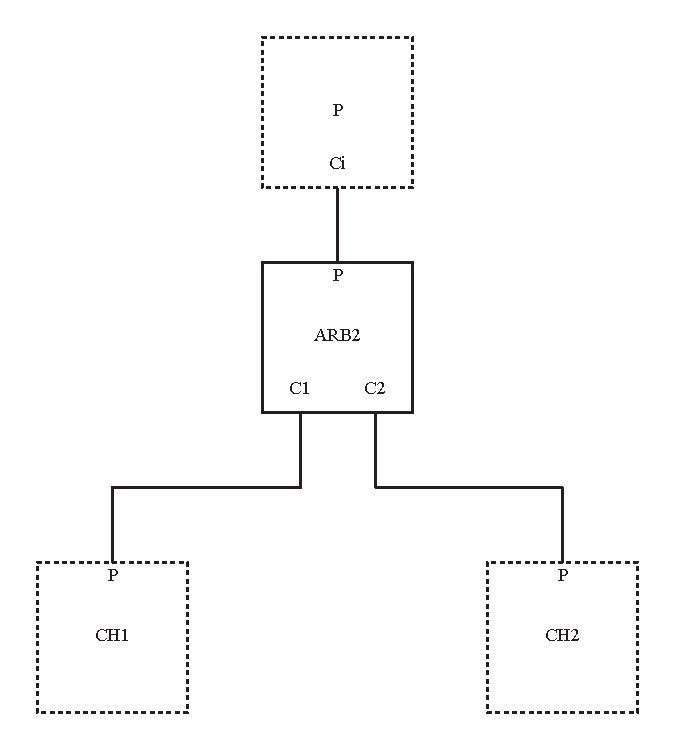
\includegraphics[width=\textwidth]{img/transmitter/arb2.pdf}
    \caption{2-input arbiter cell $ARB2$. 
    The environment consists of parent process $P$ and two children processes $CH1$ and $CH2$.}
    \label{fig:arb2}
  \end{subfigure}
  ~
  \begin{subfigure}[t]{.4\textwidth}
    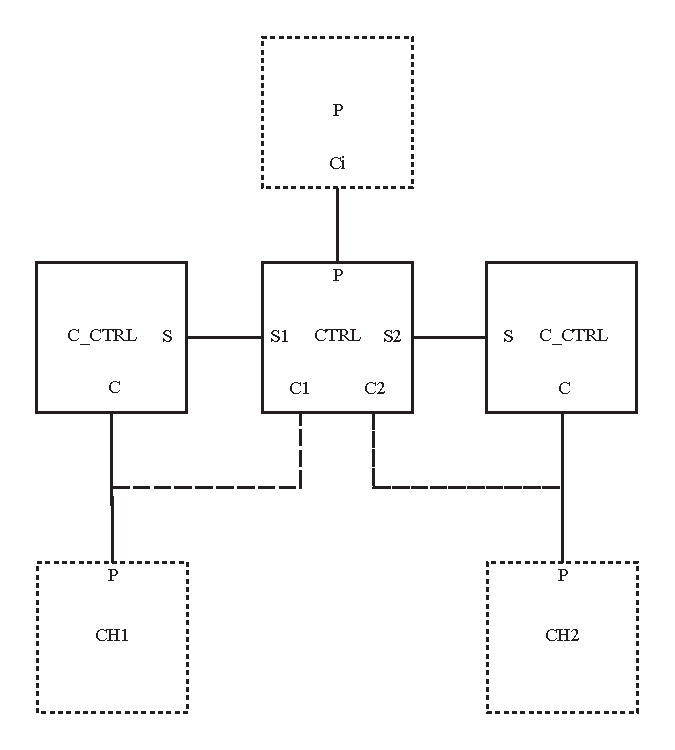
\includegraphics[width=\textwidth]{img/transmitter/ctrl.pdf}
    \caption{$ARB2$ decomposed into control and arbitration processes. 
    Dashed lines are used for probing only.}
    \label{fig:ctrl}
  \end{subfigure}
  \caption{$ARB2$ definition and initial decomposition}
\end{figure}

\noindent (see Figure~\ref{fig:arb2}). 
The arbiter cell at the top of the binary tree will have its parent port simply connected back to itself to self-acknowledge.

Based on~\cite{precise_exceptions} (section 3.3 Evaluating a Probe),
we decompose the $ARB2$ into one central control process and 
two child control processes (see Figure~\ref{fig:ctrl}).

\begin{csp}
ARB2\equiv\!CTRL\pll\!C_CTRL\pll\!C_CTRL
\end{csp}

\noindent where
\begin{csp}
CTRL\equiv
  *[[#{C1}|#{C2}->P;S1;S1;S2;S2;P]]

C_CTRL\equiv
  *[[#{C}->S;C;C;S]
    \|#{S}->S;S]]
\end{csp}

\noindent In words for $CTRL$,

\begin{tabular}[]{rl}
  $\overline{C1}\lor\overline{C2}$ & wait either child request \\
  $P$ & request parent \\
  $S1$ & signal or bypass child 1 through $C\_CTRL$ \\
  $S1$ & wait for child 1 or bypass to complete \\
  $S2$ & signal or bypass child 2 through $C\_CTRL$ \\
  $S2$ & wait for child 2 or bypass to complete \\
  $P$ & release parent \\
\end{tabular} \\ \\

By only requesting the parent once before servicing both children, $CTRL$ implements the greedy, but fair
arbitration algorithm.

\noindent In words for $C\_CTRL$,

\begin{tabular}[]{rl}
  $\overline{C}$ & wait for child request \\
  $S$ & Sync with $CTRL$ -- Indicates that child 1 should go ahead. \\
  $C$ & acknowledge child 1's request \\
  $C$ & wait for child 1 to complete \\
  $S$ & Sync with $CTRL$ -- Indicates that child 1 is finished. \\ \\
  $\vert$ & \\ \\
  $\overline{S}$ & Wait for $CTRL$ \\
  $S$ & Sync with $CTRL$ -- Indicates that child 1 should be skipped. \\
  $S$ & Sync with $CTRL$ -- Indicates that child 1 has been skipped. \\
\end{tabular} \\ \\

\noindent When a child request is present, the arbitration is biased towards seeing
the first branch's request before second branch's request.

Next, we decompose $C\_CTRL$ into gating, bypass, and arbitration processes. 

\begin{csp}
C_CTRL\equiv\!C_GATE\pll\!C_BYPASS\pll\!C_ARB
\end{csp}

\noindent where

\begin{csp}
C_GATE\equiv
  *[[#{C}->A;S;C;C;S;A]]

C_BYPASS\equiv
  *[[#{S}->A;S;S;A]]

C_ARB\equiv
  *[[#{A1}->A1;A1\|#{A2}->A2;A2]]
\end{csp}

\noindent $S$ is shared between $CTRL$. 
We introduce $C\_S$ to make the merging and splitting of the $S$ signals explicit.
(This is definition is technically incorrect, but I'm not sure at the moment how to fix it...)

\begin{csp}
C_S\equiv
  *[[S;SB,SG;SB,SG;S]]
\end{csp}

\begin{figure}
  \centering  
  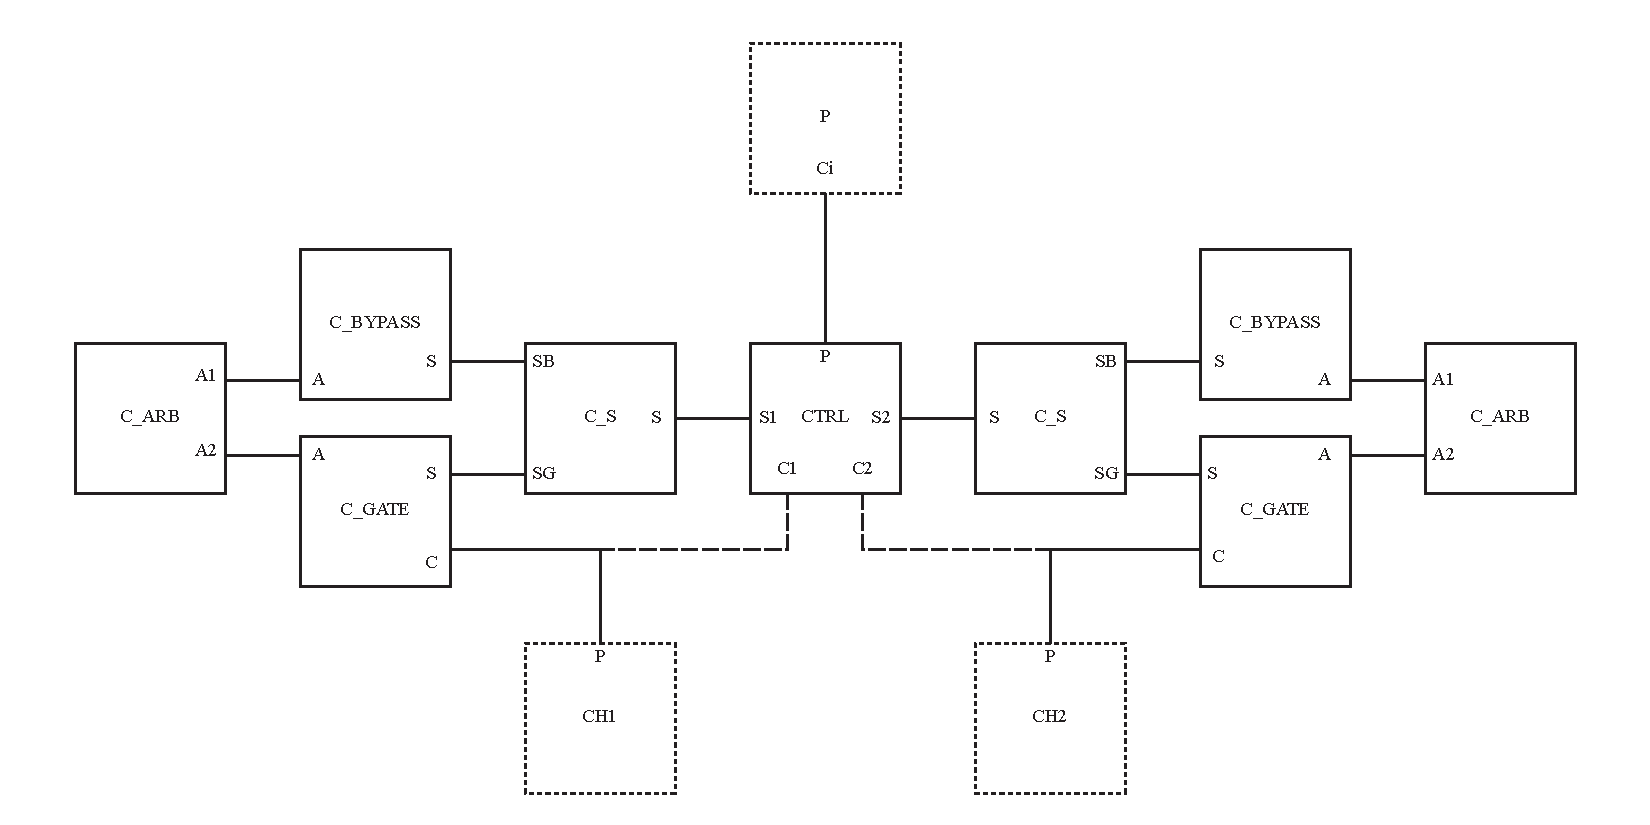
\includegraphics[width=.8\textwidth]{img/transmitter/arb.pdf}
  \caption{ARB2 decomposed into control and child subprocesses}
  \label{fig:arb2_decomp}
\end{figure}

\noindent (see Figure~\ref{fig:arb2_decomp}). Next, we pipeline $C\_GATE$ and $C\_BY\!P\!ASS$ (and fold the guards into the communications).

\begin{csp}
C_GATE\equiv
  *[C\star(A,S);C\star(A,S)]

C_BYPASS\equiv
  *[S1\star\!A;S1\star\!A]
\end{csp}

Ports used as gaurds are implemented with passive channels and
the $\star$ operator also requires that one of the channels be passive. 
These restrictions imply that $S1$ and $S2$ are active in the control process.
Likewise, $S$ is passive in the $C\_GATE$ and $C\_BY\!P\!ASS$ processes. 

Our next step is to convert the CHP into HSE and PRS, 
and as we go through the HSE and PRS we will make changes to the design to improve the implementation.
Therefore, let's collect our process definitions at this point before moving forward.

\begin{csp}
CTRL\equiv
  *[[#{C1}|#{C2}->P;S1;S1;S2;S2;P]]

C_S\equiv
  *[[S;SB,SG;SB,SG;S]]
  
C_GATE\equiv
  *[C\star(A,S);C\star(A,S)]

C_BYPASS\equiv
  *[S\star\!A;S\star\!A]

C_ARB\equiv
  *[[#{A1}->A1;A1\|#{A2}->A2;A2]]
\end{csp}

\noindent Starting with the HSE for $CTRL$,

\begin{hse}
CTRL\equiv
  *[[c1i|c2i];po+;[pi];
    s1o+;[s1i];s1o-[~s1i];
    s2o+;[s2i];s2o-;[~s2i];
    po-;[~pi]]
\end{hse}


\noindent This design will be problematic because 
we won't be able to distinguish between three states of the $CTRL$ HSE: 
between \code{[pi]} and \code{s1o$\uparrow$},
between \code{[$\neg$s1i]} and \code{s2o$\uparrow$}, and 
between \code{[$\neg$s2i]} and \code{po$\downarrow$}. 
One approach would be to introduce state variables \code{x} and \code{y}:

\begin{hse}
  *[[c1i|c2i];po+;[pi];
    s1o+;[s1i];x+;s1o-;[~s1i];y+,
    s2o+;[s2i];x-;s2o-;[~s2i];
    po-;[~pi];y-]
\end{hse}

\noindent However, state variables lead to very messy PRS implementations, 
and it's impossible to reshuffle this HSE for two reasons.
First, the $CTRL$ process must have permission from the parent before allowing the children to go ahead.
This condition is only satisfied after \code{[ri]}.
Second, the $CTRL$ process must know that its children have completed before releasing the parent.
This condition is only satisfied after \code{[$\neg$s2i]} because the $S1$ and $S2$ ports are active.

Since the active/passive constraints on port $S$ are causing us pain, let's revist the CHP.
Recall that $\star$ operators require at least one port to be passive. 
$\star$ only affects $S$ in the $C\_BY\!P\!ASS$ process. Removing the $\star$ operator yields

\begin{csp}
C_BYPASS\equiv
  *[S;A;S;A]
\end{csp}

\noindent Now we can make the \code{S1} and \code{S2} ports passive in $CTRL$:

\begin{hse}
CTRL\equiv
  *[[l1i|l2i];po+;[pi];
    [s1i];s1o+;[~s1i];s1o-;
    [s2i];s2o+;[~s2i];s2o-;
    po-;[~pi]]
\end{hse}

\noindent and reshuffle to break symmetry by delaying
\code{s1i$\downarrow$} and \code{s2i$\downarrow$} until after the
downphase of the $P$ communication.

\begin{hse}
CTRL\equiv
  *[[l1i|l2i];po+;[pi];
    [s1i];s1o+;[~s1i];
    [s2i];s2o+;[~s2i];
    po-;[~pi];s1o-,s2o-]
\end{hse}

\noindent Now we move on to $C\_GATE$ and $C\_BY\!P\!ASS$,

\begin{hse}
C_GATE\equiv    
  *[[ci];ao+,so+;[ai&si];co+;
    [~ci];ao-,so-;[~ai&~si];co-]

C_BYPASS\equiv
  *[so+;[si];ao+;[ai];
    so-;[~si];ao-;[~ai]]

C_ARB\equiv
  *[[a1i];a1o+;[~a1i];a1o-
   \|[a2i];a2o+;[~a2i];a2o-]
\end{hse}

\noindent This could deadlock in the case that a child request is present (\code{ci} is high),
and the skip process manages to grab the arbiter first because the \code{so} input to $CTRL$ 
is the wired-or of $C\_GATE$ and $C\_BYPASS$. 
Therefore, $C\_BYPASS$ must release the arbiter and controller concurrently.

\noindent CHP:

\begin{csp}
C_BYPASS\equiv
  *[S;A;S,A]
\end{csp}

\noindent HSE:

\begin{hse}
C_BYPASS\equiv
  *[so+;[si];ao+;[ai];
    so-,ao-;[~si&~ai]]
\end{hse}

\noindent Note that now the $GATE$ process will never actually be skipped because
the $SKIP$ process cannot finish until \code{s1i} goes low. Since \code{s1o} is
a wired or, \code{s1i} will not go low until both \code{s1o} lines go low.

At this point, we can reshuffle $CTRL$ to break its symmetry by moving
the \code{s1i$\downarrow$} and \code{s2i$\downarrow$} to after the
downphase of the $R$ communication.

\begin{hse}
  *[[l1i|l2i];ro+;[ri];
    [s1o];s1i+;[~s1o];
    [s2o];s2i+;[~s2o];
    ro-;[~ri];s1i-,s2i-]
    
  *[[l1i];a1lo+,s1o+;[a1li&s1i];l1o+;
    [~l1i];a1lo-,s1o-;[~a1li&~s1i];l1o-]
  *[s1o+;[s1i];a1so+;[a1si];
    s1o-,a1so-;[~s1i&~a1si]]
  *[[a1lo];a1li+;[~a1lo];a1li-
   \|[a1so];a1si+;[~a1so];a1si-]
\end{hse}

\noindent This corresponds to the CHP

\begin{csp}
  *[[#{L1}|#{L2}->R;S1;S1\star(S2;S2\star\!R)]]

  *[L1\star(A1l,S1);L1\star(A1l,S1)]
  *[S1;A1s;S1,A1s]
  *[[#{A1l}->A1l;A1l\|#{A1s}->A1s;A1s]]
\end{csp}

\noindent The PRS for \code{CTRL}:

\begin{prs2}
ri & s1o -> s1i+
~ri -> s1i-

s1i & ~s1o & s2o -> s2i+
~ri -> s2i-

l1i | l2i -> ro+
s2i & ~s2o -> ro-
\end{prs2}

\begin{hse}
C_S\equiv
  *[[si];sgo+,sbo+;[sgi|sbi];so-]
  
C_GATE\equiv
  *[[ci];ao+;[si];so+;[ai];co+;
    [~ci];ao-;[~si];so-;[~ai];co-]

C_BYPASS\equiv
  *[[s1o];a1so+;[a1si];s1i+;
    [~s1o];a1so-;[~a1si];s1i-]

C_ARB\equiv
  *[[a1lo];a1li+;[~a1lo];a1li-
   \|[a1so];a1si+;[~a1so];a1si-]
\end{hse}


\noindent The PRS for \code{CH1\_GATE}:

\begin{prs2}
l1i -> a1lo+, s1o+
~l1i -> a1lo-, s1o-

a1li & s1i -> l1o+
~a1li & ~s1o -> l1o-
\end{prs2}

\noindent The PRS for \code{CH1\_BYPASS}:

\begin{prs2}
~s1i&~a1si -> s1o+
s1i -> a1so+
a1si -> s1o-, a1so-
\end{prs2}

\noindent The PRS for \code{CH1\_ARB}:

\begin{prs2}
a1lo & _a1si -> _a1li-
~a1lo | ~_a1si -> _a1li+

~_a1li & _a1si -> a1li+
_a1li -> a1li-

a1so & _a1li -> _a1si-
~a1so | ~_a1li -> _a1si+

~_a1si & _a1li -> a1si+
_a1si -> a1si-
\end{prs2}

\noindent which is just a standard 2-input arbiter (see section~\ref{subsec:arb})
with inputs \code{a1lo} and \code{a1so}

%%%%%%%%%%%%%%%%%%%%%%%%%%%%%%%%%%%%%%%%%%%%%%%%%%%%%%%%%%%%%%%%%%%%%%%%%%%%%%%
\section{Scratch}

Here is scratch space and some failed designs

%%%%%%%%%%%%%%%%%%%%%%%%%%%%%%%%%%%%%%%%%%%%%%%%%%%%%%%%%%%%%%%%%%%%%%%%%%%%%%%
\subsection{A Better Arbiter}

Starting with

\begin{csp}
ARB2\equiv*
  *[[#{L1}->R;L1;L1;R
    \|#{L2}->R;L2;L2;R]]
\end{csp}

we split out the arbitration into a separate process.

\begin{csp}
ARB2\equiv
*[[#{L1}->A1;R;L1;L1;R;A1]] \pll
*[[#{L2}->A2;R;L2;L2;R;A2]] \pll
*[[#{A1}->A1;A1\|#{A2}->A2;A2]]
\end{csp}

This arbiter is not greedy and returns the token to the parent after servicing a child.
To make it greedy yet fair, we split out communication with the parent arbiter cell into a separate process.

\begin{csp}
ARB2\equiv
  *[[#{L1}->A1;R1;L1;L1;A1;R1)]] \pll
  *[[#{L2}->A2;R2;L2;L2;A2;R2)]] \pll
  *[[#{A1}->A1;A1\|#{A2}->A2;A2]]\pll
  *[[#{R1}|#{R2}->R;
    [#{R1}->R1;R1\|~#{R1}->skip],
    [#{R2}->R2;R2\|~#{R2}->skip];
    R]]
\end{csp}

The parent communication process implements a greedy algorithm because once it acquires the token from the parent,
it will not return the token until both children have been serviced (if both have requested). 
The algorithm is fair because each child will only be serviced at most once for posession of the token.
The parent communication process can signal children processes in parallel because aribtration is handled by the arbitration process.
We use synchronizers (see section~\ref{subsec:sync}) enabled by the parent request to ensure that selection guards are mutually exclusive.


\begin{csp}
ARB2\equiv
  *[[#{L1}->A1;R1;L1;L1;A1;R1)]] \pll
  *[[#{L2}->A2;R2;L2;L2;A2;R2)]] \pll
  *[[#{A1}->A1;A1\|#{A2}->A2;A2]]\pll
  *[[#{R1}|#{R2}->R;
    [#{R1'}->R1;R1[]~#{R1'}->skip],
    [#{R2'}->R2;R2[]~#{R2'}->skip];
    R]]
\end{csp}
where probes on $R1$ and $R2$ have been replaced with probes on $R1'$ and $R2'$, respectively. 
These are synchronized versions of their respective signals.

Next, we make the 2-phase portions of each 4-phase communication explicit so we can pipeline them.
Since each communication is paired, it's straightforward to assign the first and second as the first and second
2-phase communications of a 4-phase protocol. 

\begin{csp}
ARB2\equiv
  *[[#{L1}->A1+;R1+;L1+;L1-;A1-;R1-]] \pll
  *[[#{L2}->A2+;R2+;L2+;L2-;A2-;R2-]] \pll
  *[[#{A1}->A1+;A1-\|#{A2}->A2+;A2-]]\pll
  *[[#{R1}|#{R2}->R+;
    [#{R1'}->R1+;R1-[]~#{R1'}->skip],
    [#{R2'}->R2+;R2-[]~#{R2'}->skip];
    R-]]
\end{csp}

We pipeline the arbitration and parent requests for speed.

\begin{csp}
ARB2\equiv
  *[[#{L1}->A1+,R1+;L1+;L1-\star(A1-,R1-)]] \pll
  *[[#{L2}->A2+,R2+;L2+;L2-\star(A2-,R2-)]] \pll
  *[[#{A1}->A1+;A1-\|#{A2}->A2+;A2-]]\pll
  *[[#{R1}|#{R2}->R+;
    [#{R1'}->R1+;R1-[]~#{R1'}->skip],
    [#{R2'}->R2+;R2-[]~#{R2'}->skip];
    R-]]
\end{csp}

or alternatively expressed with fewer guards as

\begin{csp}
ARB2\equiv
  *[L1+\star(A1+,R1+);L1-\star(A1-,R1-)] \pll
  *[L2+\star(A2+,R2+);L2-\star(A2-,R2-)] \pll
  *[[#{A1}->A1+;A1-\|#{A2}->A2+;A2-]]\pll
  *[[#{R1}|#{R2}];R+;
    [#{R1'}->R1+;R1-[]~#{R1'}->skip],
    [#{R2'}->R2+;R2-[]~#{R2'}->skip];
    R-]
\end{csp}

The HSE is given by

\begin{hse}
*[[l1i];a1o+,r1o+;[a1i&r1i];l1o+;
  [~l1i];a1o-,r1o-;[~a1i&~r1i];l1o-]
*[[l2i];a2o+,r2o+;[a2i&r2i];l2o+;
  [~l2i];a2o-,r2o-;[~a2i&~r2i];l2o-]
  
*[[a1o];a1i+;[~a1o];a1i-
 \|[a2o];a2i+;[~a2o];a2i-]
 
*[[r1o|r2o];ro+;[ri];
  [[r1o'];r1i+;[~r1o];r1i-[][_r1o']],
  [[r2o'];r2i+;[~r2o];r2i-[][_r2o']];
  ro-;[~ri]]
\end{hse}

The arbiter and synchronizer processes are standardized (see sections~\ref{subsec:arb} and~\ref{subsec:sync}), 
so we will omit their PRS here. First we develop the PRS for the children communication processes

\begin{prs2}
l1i->a1o+,r1o+
~l1i->a1o-,r1o-

a1i&r1i->l1o+
~a1i&~r1i->l1o-

l2i->a2o+,r2o+
~l2i->a2o-,r2o-

a2i&r2i->l2o+
~a2i&~r2i->l2o-
\end{prs2}

To make these CMOS implementable, we invert the senses of the $L1$ and $L2$ ports.

\begin{prs2}
~_l1i -> a1o+, r1o+
_l1i -> a1o-, r1o-

a1i & r1i -> _l1o-
~a1i & ~r1i -> _l1o+

~_l2i -> a2o+, r2o+
_l2i -> a2o-, r2o-

a2i & r2i -> _l2o-
~a2i & ~r2i -> _l2o+
\end{prs2}

Next we develop the PRS for the parent communication process

\begin{prs2}
~ri & (r1o | r2o) -> ro+
~r1o & ~r2o -> ro-

~ri & r1o' -> r1i+

~ri & r2o' -> r2i+

\end{prs2}

This is where things became really complicated and we abandoned this design.



\end{document}
